%% LyX 2.0.5.1 created this file.  For more info, see http://www.lyx.org/.
%% Do not edit unless you really know what you are doing.
\documentclass[french]{article}
\usepackage[T1]{fontenc}
\usepackage[utf8]{inputenc}
\usepackage{geometry}
\geometry{verbose}
\usepackage{float}
\usepackage{graphicx}
\usepackage{babel}
\makeatletter
\addto\extrasfrench{%
   \providecommand{\og}{\leavevmode\flqq~}%
   \providecommand{\fg}{\ifdim\lastskip>\z@\unskip\fi~\frqq}%
}

\makeatother
\begin{document}

\title{Projet de Programmation Comparée \\
~\\
 \og Interfaces Utilisateurs \fg{}\\
~}


\author{Nicolas Chenciner, Melody Méaulle, David Bühler}

\maketitle
\vphantom{}

\begin{center}
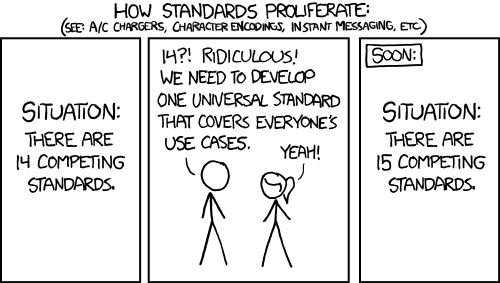
\includegraphics[scale=0.75]{images/standards}
\par\end{center}

\newpage{}


\section*{Introduction}

Introduction - blablabla

Nous allons introduire un exemple suivi, qui sera utilisé tout au
long de ce rapport. Le but est d'illustrer nos remarques et idées
grâce à un cas d'étude simple. \\
L'application considérée se contente de gérer une liste et un compteur.
Elle est munie d'une interface graphique constituée d'une fenêtre,
ainsi que de deux vues, ou panneaux, qui ne sont pas visibles en même
temps, mais avec la possibilité de passer de l'une à l'autre. Ces
vues seront affichées, lorsque visibles, dans la fenêtre précédemment
mentionnée. \\
L'une des deux vues offre une représentation et des outils de modification
de la liste gérée par l'application alors que l'autre se charge du
compteur. \\
Deux menus sont présents, l'un attaché à la fenêtre et l'autre \og flottant \fg{}
accessible via une interaction entre l'utilisateur et l'interface.\\
\medskip{}


\begin{figure}[H]
\begin{centering}
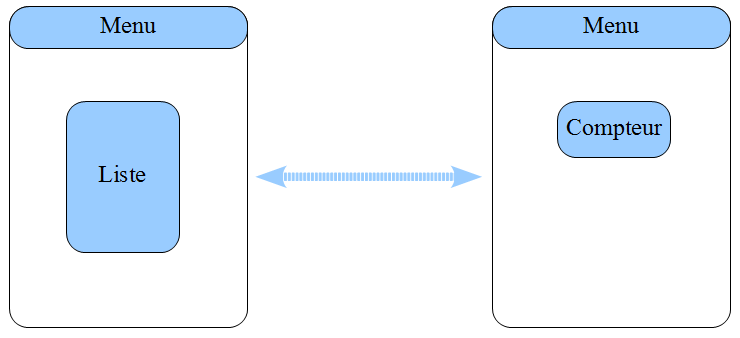
\includegraphics[scale=0.5]{images/base-exemple-projet}
\par\end{centering}

\caption{Concept de base}
\end{figure}



\section{Qu'est ce qu'une interface utilisateur et comment en programmer}

Nous allons aborder dans cette partie différents points nous permettant
de définir les concepts et mécanismes importants mis en jeu lors de
la conception, mais aussi de l'utilisation, d'une interface graphique.
Comme nous le verrons, les deux aspects sont fortement liés.


\subsection{Définition des concepts liés à la création d'interface utilisateur}

La compréhension de la notion d'interface utilisateur passe par une
définition des utilisateurs et des outils de conception sollicités.


\subsubsection*{Les utilisateurs}

Avant toute analyse ou réflexion, il est important de définir qui
sont les utilisateurs du système considéré. Nous distinguerons deux
catégories d'utilisateurs et nous utiliserons la terminologie suivante
: \medskip{}

\begin{itemize}
\item \textbf{Programmeur :} il est notre cible directe, c'est lui qui utilisera
les outils que nous allons développer afin de construire des interfaces
utilisateurs (nous parlerons ici essentiellement d'interfaces graphiques)
pour ses applications.\medskip{}

\item \textbf{Utilisateur application : }il est l'utilisateur des produits
développés par le programmeur, il est n'est pas notre cible directe
mais il est important de ne pas l'oublier.
\end{itemize}
~

Une approche orientée utilisateur sera adoptée lors de la conception,
les besoins étant différents pour les deux catégories d'utilisateurs
considérées, nous ferons bien attention de prendre en compte les deux
points de vue. En particulier, celui de l'utilisateur application
doit être pris en compte même s'il sera la cible du système développé
par le programmeur et non directement celle du notre. Ses besoins
doivent nous permettre de mieux déterminer les éléments nécessaires
aux programmeurs pour satisfaire à ses exigences envers le produit
fini.


\subsubsection*{Conception - génie logiciel}

La conception d'une interface utilisateur doit être centrée autour
des deux catégories d'acteurs définies précédemment, l'utilisation
du modèle de conception centré utilisateur semble alors tout à fait
correspondre aux besoins. \\
Ce dernier est itératif, chaque itération étant composée des trois
phases suivantes :\medskip{}

\begin{itemize}
\item \textbf{Analyse :} on analyse les besoins des acteurs du système,
un panel représentatif d'utilisateurs des deux catégories concernées
doit être constitué afin d'établir les dits besoins.\medskip{}

\item \textbf{Conception :} un prototype doit être conçu en fonction des
besoins établis à l'étape précédente. Chaque prototype servira le
plus souvent de base à celui à l'étape suivante\medskip{}

\item \textbf{Évaluation :} sur la base du prototype réalisé, une évaluation
est faite. Le procédé étant itératif, cette évaluation servira de
base à la modification des besoins de la première étape de l'itération
suivante. \medskip{}

\end{itemize}
Afin de mener à bien ces trois phases, il est nécessaire d'établir
des critères d'évaluation qui serviront aussi de base à l'élaboration
des besoins. \medskip{}

\begin{itemize}
\item \textbf{Pour l'utilisateur application :}\medskip{}


\begin{itemize}
\item \textbf{Facilité d'utilisation :} la vitesse d'apprentissage, l'aide
extérieure nécessaire ainsi que le nombre d'erreurs commises lors
d'un test sont de bons indicateurs. Il faut de plus prendre en compte
les différents niveaux de compétences parmi les utilisateurs.\medskip{}

\item \textbf{Correction des erreurs }: la possibilité d'annuler une action
est indispensable (cf. partie 3.1)\medskip{}

\item \textbf{Rapidité :} le temps de réponse de l'interface doit être faible.
Il faut définir par des tests quel est le délai admissible avant réponse
et quel est le meilleur moyen de faire patienter l'utilisateur application.\medskip{}

\item \textbf{Aspect visuel }: il doit être agréable et clair. (nous pourrions
parler d'aspect sensoriel pour être plus général, mais nous allons
nous concentrer sur les interfaces graphiques)\medskip{}

\end{itemize}
\end{itemize}
~
\begin{itemize}
\item \textbf{Pour le programmeur :}\medskip{}


\begin{itemize}
\item \textbf{Expressivité :} une bonne expressivité des langages / outils
utilisés est nécessaire, un code clair et précis est plus agréable.
De plus il est important d'essayer de rendre la programmation via
le système intuitive.\medskip{}

\item \textbf{Adaptabilité :} une bonne capacité d'adaptation aux différents
support ainsi qu'une portabilité sont nécessaires.\medskip{}

\item \textbf{Sûreté :} un code qui compile doit être un code qui marche.\medskip{}

\item \textbf{Debugging :} des outils de debugging doivent être fournis,
une analyse statique de pertinence serait un plus (détecter le maximum
d'absurdités comme des éléments inutiles par exemple).\medskip{}

\item \textbf{IDE :} une intégration aux IDE populaires est nécessaire,
la création d'un IDE spécifique peut être envisagé.\medskip{}

\item \textbf{Efficacité :} les critères en terme de consommation des ressources
de la machine doivent être étudiés.\medskip{}

\end{itemize}
\end{itemize}
~

Tout au long de ce processus de conception, des outils issus du génie
logiciel vont nous aider, en voici trois particulièrement adaptés
:

~
\begin{itemize}
\item \textbf{Scénarios / diagrammes de cas d'utilisation :} leur utilisation,
combinée aux critères mis en place ci-dessus, nous permettra à la
fois d'établir les besoins et d'effectuer des tests choisis dans le
cadre de l'évaluation. \medskip{}

\item \textbf{Diagrammes relationnels - diagrammes de classes :} même si
elle ne doit pas nous aveugler, la programmation orientée objet est
adaptée au sujet. La réflexion à mener quant à l'organisation du système
considéré se prête remarquablement bien à l'utilisation de ces outils.
De plus, ils nous permettent, à un autre niveau, de nous mettre à
la place du programmeur qui devra concevoir une interface en utilisant
notre système.\medskip{}

\item \textbf{Design pattern :} l'implémentation ``native'' de comportements
génériques, typiquement pour les interactions entre l'utilisateur
application et l'interface créée, permet à la fois de faciliter l'utilisation
de notre système par le programmeur mais aussi d'établir un cadre
sûr pour les les dites interactions. La partie 3.1 de ce rapport est
un exemple de ce principe.
\end{itemize}

\subsection{Division du travail}

La conception d'une interface graphique par dessus un moteur d'application
peut se diviser en quatre étapes ; une bibliothèque graphique devrait
fournir des outils adéquats pour chacune, et minimiser les interdépendances
entre elles.


\paragraph{Communication entre le moteur et l'interface}

Une bibliothèque graphique doit fournir des outils adaptées à la \og communication \fg{}
entre l'interface et le moteur logique de l'application
\begin{itemize}
\item affichage : ensemble des données du moteur affichées (sous diverses
formes) par l'interface ;
\item actions : ensemble des actions de l'utilisateur modifiant l'état des
données. 
\end{itemize}
Cette partie du code pose les bases de ce qu'utilisera l'interface,
ce à quoi elle est destinée, mais doit demeurer indépendante de son
implémentation réelle, des éléments graphiques concrets utilisés pour
la fabriquer, et de la plateforme à laquelle elle est destinée.


\paragraph{Éléments de l'interface}

Il s'agit ensuite de définir les éléments de l'interface graphique
qui serviront de support aux données et possibilités définis précédemment
; ceux-ci devront donc interagir avec le système logique de communication,
et non directement avec le moteur de l'application.

Ils sont évidemment dépendants de la plateforme à laquelle l'interface
est destinée : les raccourcis clavier d'un ordinateur seront remplacés
par des gestes tactiles sur une tablette, par exemple.\\


La bibliothèque se doit de définir un panel aussi vaste que possible
d'éléments graphique à disposition du développeur.

Notons que ces éléments ne sont pas forcément tous graphiques (lecture
d'un texte ou commande vocale).


\paragraph{Placement des éléments}

Les éléments doivent ensuite être assemblés pour former une interface
cohérente et fonctionnelle. À cette fin, de nombreux outils doivent
être présents pour le développeur : divers \og layout \fg{} permettant
diverses dispositions des éléments au sein d'une même fenêtre, gestion
intelligente des redimensionnements, système d'onglets, éléments permettant
le zoom et défilement, fenêtres pop-up, panneaux d'options, etc.

Une telle configuration s'effectue évidemment sur un ensemble d'éléments
de l'interface déjà défini, dont la taille et l'aspect graphique doivent
également pouvoir être éventuellement personnalisés au cas par cas.\\


Par ailleurs, le développeur peut laisser une partie de cette configuration
de l'interface à disposition de l'utilisateur final : lui permettre
de choisir les éléments présents d'une barre d'outils, ou le placement
de celle-ci sur certains bords de la fenêtre, tout en excluant certaines
autres modifications, le menu restant toujours identique.

Enfin, la forme finale d'une interface doit pouvoir être aisément
enregistrée, et il doit être possible pour l'utilisateur final de
passer d'une configuration à une autre s'il en existe plusieurs possibles
pour une application donnée.


\paragraph{Aspect général}

Enfin, la bibliothèque peut permettre au développeur de modifier l'aspect
général de son interface, en personnalisant l'aspect d'un type d'éléments
graphiques. Cette dernière partie est optionnelle, mais si la possibilité
existe, elle doit être indépendante des trois premières : modifier
l'aspect général des boutons ne doit pas impacter le code de l'interface
déjà écrite.


\subsection{Exemple suivi}

Dans cette première itération de notre exemple suivi, nous n'allons
pas forcement être exhaustifs, mais nous allons essayer d'aborder
les points importants pour mener à bien la réalisation de notre exemple.
Nous allons commencer par étudier les besoins de l'utilisateur application.\medskip{}

\begin{itemize}
\item \textbf{Annulation :} il est nécessaire de pouvoir annuler une opération
effectuée via l'interface graphique sur la liste ou le compteur. On
peut aussi vouloir annuler un changement de vue.\medskip{}

\item \textbf{Adaptativité - facilité d'utilisation :} le passage d'une
vue à l'autre doit se faire via un outil adapté au support. Par exemple,
un bouton sur chaque panneau avec un raccourci associé pour une paire
clavier / souris mais une \og gesture \fg{} sur une tablette ou
un smartphone. \\
Il en est de même pour toutes les actions proposées par l'interface,
y compris la gestion du menu flottant (apparition au clic droit pour
le clavier / souris et utilisation d'une \og touche \fg{} à deux
doigts pour une tablette ou un smartphone). \\
La position du menu attaché à la fenêtre doit dépendre du support,
sur un smartphone la taille relativement petite de l'écran oblige
à prévoir un emplacement plus adapté, voir même de ne pas l'afficher.\medskip{}

\item \textbf{Rapidité :} le changement de vue et l'apparition du menu flottant
doivent être rapides, il ne faut surtout pas donner l'impression à
l'utilisateur qu'il est en attente passive. \\
Les opérations sur la liste et le compteur peuvent être soumises à
des contraintes au niveau de la partie logique de l'application, l'interface
doit être capable d'afficher une barre de progression par exemple
pour montrer qu'une action est en cours.\medskip{}

\end{itemize}
Nous pouvons alors définir les exigences du programmeur qui en découlent
:\medskip{}

\begin{itemize}
\item \textbf{Liste - compteur :} avoir la possibilité de lier directement
une liste ou un compteur à sa représentation graphique sans que le
programmeur ait à lui même définir un protocole de mise à jour et
l'implémenter est nécessaire.\medskip{}

\item \textbf{Adaptativité : }le programmeur ne doit pas avoir à programmer
plusieurs interfaces juste pour changer le bouton de changement de
vue en \og gesture \fg{} ou changer l'emplacement du menu. \\
Afin de faciliter l'adaptation du style graphique au support, il faut
permettre au programmeur de ne pas avoir à définir \og à la main \fg{}
les emplacements de la liste, du compteur, des menus ainsi que des
boutons, si boutons il y a, de changement de vue.
\end{itemize}

\section{Analyse de l'existant}

Une analyse de l'existant, en conjonction avec notre précédente analyse
des besoins nous permettra de tenter dans la suite d'apporter des
solutions aux problèmes actuels.


\subsubsection*{Difficultés de la programmation d'interfaces graphiques}

Programmer une interface graphique entièrement à la force du poignet
n'est guère agréable, pour différentes raisons :
\begin{itemize}
\item Apprendre à programmer une interface graphique en utilisant l'une
ou l'autre API existante peut se révéler fastidieux et complexe. En
particulier, nous remarquerons que GTK+ tend à être plus laid et moins
intuitif que des bibliothèques reposant sur le modèle objet, comme
Qt ou Swing.
\item Dans tous les cas, la programmation est longue, répétitive et, à de
rares exceptions (TkInter ?), extrêmement verbeuse.
\item Ceci est, a priori, dû à ce que Swing, GTK+, Qt et les autres bibliothèques
reposent entièrement sur un modèle de widgets : des composants imbriqués
les uns dans les autres de façon quasi-infinie, qu'on doit tous définir,
paramétrer et placer manuellement. On parle d'ailleurs de widget toolkit
pour définir les bibliothèques permettant de construire des interfaces
graphiques.
\end{itemize}

\subsubsection*{Environnements de développement}

Différents environnements de développement intégré (IDE) plus ou moins
sophistiqués, tels que QtCreator/QtDesigner ou Glade, peuvent faciliter
la création d'interfaces graphiques, mais il est toujours nécessaire
de savoir coder et de comprendre l'API utilisé avant de pouvoir vraiment
en tirer parti. 

MacOS propose, avec XCode et différents outils comme Cocoa, une vision
intéressante -> à développer.


\subsubsection*{Portabilité}

Qt est disponible en natif sur la plupart des systèmes d'exploitation
existants, et notamment les systèmes embarqués, incluant Android,
VxWorks ou encore BlackBerry OS. GTK+ lui n'est disponible que sur
les systèmes de bureaux majeurs : Windows, MacOS, Linux/Unix.\\


Swing offre une définition de la portabilité différente de celle de
Qt et GTK+ : en effet, la bibliothèque n'est utilisable qu'en Java,
mais celui-ci étant multiplateforme, Swing devient fonctionnel sur
tout système sur lequel Java est disponible. En revanche il ne peut
être utilisé qu'en java, alors que Qt et GTK+ disposent de \og bindings \fg{}
vers de nombreux autres langages. Nativement, Qt est une bibliothèque
C++, et dispose de bindings Java, Perl, Python, PHP ou encore Ruby.
GTK+ est une bibliothèque C, disposant de bindings C++, Java, Perl,
Python, PHP, et Ruby mais aussi C\# et Javascript ; GTK+ dispose même
d'un binding Vala, un langage spécifiquement créé pour les développeurs
de Gnome, basé sur C\# et qui compile vers C !\\


Les éditeurs d'interfaces de GTK+ et Qt, respectivement Glade et QtDesigner,
permettent d’enregistrer les interfaces créées sous forme de fichier
XML. Le concept est intéressant puisqu'il permet de \og porter \fg{}
une interface dans différents langages, sans avoir à modifier le code.
Cela aide donc à séparer le fond et la forme du logiciel. Il existe
par ailleurs des langages de descriptions d'interface graphique basés
sur XML (XAML et XUL par exemple) -> à approfondir.


\subsubsection*{Adaptation des interfaces à leur environnement}

Les différents outils dédiés à la programmation d'interfaces graphiques,
en particulier Swing, nous promettent souvent de s'adapter au \emph{look
and feel} de l'environnement dans lequel l'application est exécutée.
Si l'idée est bonne puisqu'elle permettrait aux programmeurs d'obtenir
des applications parfaitement intégrées dans les différents OS sans
avoir à faire quoique ce soit de particulier, le résultat est en pratique
souvent aléatoire et rarement esthétique. {[}Screenshots{]}


\paragraph{L'exemple particulier du HTML / CSS\protect \\
}

Bien que n'étant pas fait pour la création d'interfaces graphiques
stricto sensu, le couple \textsc{html css }propose une approche intéressante
de la conception d'une interface web : séparer le style de la description
des éléments.

Le but est ici de pouvoir afficher un même contenu sous différentes
formes, par choix de l'utilisateur sur les sites qui le proposent,
ou selon le support utilisé : un document \textsc{html} peut utiliser
différentes feuilles de styles et définir laquelle sera utilisée selon
le média sur lequel il sera affiché, et un document \texttt{\textsc{css}}
peut lui-même choisir d'afficher un élément différemment selon le
support, par exemple pour optimiser le rendu d'une page web à l'impression.\\


Néanmoins on a un problème similaire à celui des interfaces graphiques
qui n'ont pas le même rendu sous différents environnements : tous
les navigateurs n'interprètent pas le \textsc{css }de la même manière
alors qu'ils le devraient.

De plus, le concept de \og boites dans des boites \fg{} est toujours
présent (les balises imbriquées du \textsc{html}).


\subsubsection*{Performances}

Si autrefois GTK+ était célèbre pour être plus rapide que Qt (ce qui
apparemment était dû au vieux compilateur utilisé par Qt ?), les deux
ont aujourd'hui des performances similaires que ce soit au niveau
de la mémoire ou du CPU, ce n'est donc plus un critère pour les départager.


\subsubsection*{Debugging}

Le debugging des interfaces graphiques est particulièrement peu aisé,
et aucun outil n'offre d'analyse statique qui permettrait de détecter
\emph{a priori} qu'un élément est invisible ou inaccessible. Cette
difficulté n'est pas seulement dépendante de la bibliothèque utilisée,
mais aussi et surtout du nombre d'interactions possibles avec l'interface,
et de séquencements possibles. Un \og petit \fg{} programme comme
WordPad aurait ainsi 325 opérations possibles via l'interface graphique.

Il existe des outils entièrement dédiés au debugging d'interfaces
graphiques : Java intègre par exemple dans son API une classe (Robot)
permettant d'aider à l'automatisation des tests d'interfaces AWT.
Eclipse dispose d'un plugin SWTBot dédié au test des interfaces SWT
alors qu'il intègre évidemment déjà un debugger Java... Les IDE évoqués
ont aussi leurs outils de debugging.


\subsubsection*{Conclusion ?}

\textbf{Exemple suivi :} (si le programmeur veut satisfaire aux besoins
d'aptabilité de l'utilisateur application, il va être obligé de définir
plusieurs interfaces différentes, pour les actions, faire en sorte
que les raccourcis dans le menu, les boutons ou autres gestures soient
associés à des actions est possible en swing, mais assez moche et
peu pratique, de plus elles ne sont pas assez évoluées pour permettre
une annulation par la suite. La mise à jour de la liste de du compteur
ne sont pas gérés de façon pratique par SWING, le faire manuellement
est finalement la solution employée)


\section{Outils à développer}

Nous allons exposer dans cette partie nos quatre principales idées
d'innovation pour la conception d'interfaces graphiques.


\subsection{Actions}

Une librairie graphique se doit de fournir une représentation des
\emph{actions} que l'utilisateur peut accomplir. Fondamentalement,
il s'agit d'une fonction qui a accès au moteur de l'application, contrairement
à l'interface proprement dite, mais d'autres mécanismes internes s'y
greffent.

Ces \emph{actions} sont indépendantes des éléments graphiques concrets
qui l'implémentent, et donc en particulier de la plateforme sur laquelle
tourne l'interface utilisateur.

Toute intervention de l'utilisateur final sur le système de l'application
doit passer par une \emph{action} telle que définie par la librairie.\\


Deux principes nous guident :
\begin{itemize}
\item La façon dont l'utilisateur accomplit cette action n'a aucune importance
; l'action n'a pas besoin de savoir qu'elle a été déclenchée par un
bouton, une entrée de menu, un raccourci clavier, une commande vocale,
ou même comme conséquence automatique d'une autre action.
\item Tous les paramètres des éléments graphiques liés à une action doivent
être \og transférés \fg{} à l'action si possible, tels que :

\begin{itemize}
\item les raccourcis claviers, noms, descriptions, textes d'aide ou icônes
associés à une action ;
\item la possibilité d'accomplir l'action (qui déterminera si le bouton
ou l'entrée de menu sont actifs ou non, par exemple).
\end{itemize}
\end{itemize}
~

Ce mécanisme d'action fourni par la librairie graphique doit être
doté d'un pattern \og observer \fg{}, permettant à d'autres éléments
d'être notifié du déclenchement de l'action.

Les actions doivent pouvoir être aisément composées, afin de permettre
au développeur de n’implémenter que les interactions minimales avec
son système, tout en proposant à l'utilisateur final des fonctionnalités
simples autant qu'avancés, résultant éventuellement de combinaisons
complexes de ces briques de base.

Enfin, les actions effectuées doivent pouvoir être enregistrées, afin
d'en conserver un historique. Idéalement, si chaque action dispose
également d'une fonction \og inverse \fg{} permettant d'annuler
ses effets, la bibliothèque graphique peut fournir elle-même la fonctionnalité
\og undo / redo \fg{}, aujourd'hui devenue indispensable à toute
interface moderne.


\subsection{Bindings}

Très souvent, l'intervention de l'utilisateur modifie des valeurs
internes au moteur de l'application ; parfois néanmoins, l'inverse
peut être également utile : la modification d'une valeur du moteur
de l'application modifie l'état d'un élément de l'interface. Il s'agit
alors de modéliser efficacement la liaison d'une propriété d'un élément
graphique à une valeur de la logique interne de l'application.\\


Voici quelques exemples qui pourraient se révéler utiles au développement
d'une interface :
\begin{itemize}
\item progression d'une opération affichée par une barre de progression
;
\item possibilité d'effectuer une action liée à un booléen, impliquant l'apparence
des éléments graphiques qui lui sont liés (actifs ou non) ;
\item champs d'un label liée à une chaîne de caractère, position d'un curseur
liée à une valeur numérique ;
\item contenu d'un panneau lié à une image dynamiquement déterminée par
le moteur applicatif.\\

\end{itemize}
Si l’élément graphique peut être édité par l'utilisateur, la liaison
doit être effective dans les deux sens : le changement du champs du
label par l'utilisateur doit modifier la valeur de la chaîne de caractère
en interne, tout autre changement de la valeur doit être immédiatement
répercuté dans l'affichage, comme dans le cas de la barre d'url des
navigateurs internet (qui est évidemment actualisé en cas de redirection,
ou si l'utilisateur utilise un autre moyen pour parvenir sur un page
web).\\


À cette fin, la librairie graphique peut proposer des représentations
des types simples \og pertinents \fg{} comprenant un pattern observer
à destination des éléments de l'interface ; la liaison d'une propriété
graphique à la valeur deviendrait alors immédiate et transparente
pour le développeur. 

L'inconvénient est que le moteur de l'application doit alors utiliser
la librairie graphique pour implémenter de telles valeurs.


\subsection{Le modèle relationnel}

Les différents éléments d'une interface utilisateur doivent être mis
en relation les uns avec les autres afin de former un tout cohérent.
Le principe le plus basique, qui est celui du modèle à widget évoqué
dans la partie 2, est de ne considérer qu'une seule relation : la
relation de parenté entre le contenant et le contenu.

Il serait cependant intéressant de pouvoir définir plus finement les
relations entre ces différents éléments, plus précisément, l'idée
serait de ne pas avoir à décrire l'emplacement d'un élément par rapport
à un autre, mais plutôt les relations entre ces éléments, un peu à
la manière du couple HTML / CSS.

Un premier exemple de relation autre qu'une relation de parenté est
la relation \og menu \fg{} qui est, à un niveau basique, présente
dans Swing : pour certains éléments il est possible de définir un
menu sans avoir à spécifier que ce dernier est contenu dans l'élément
demandeur. Il y a une relation de \og menu \fg{} entre ces deux
éléments et non une relation directe de positionnement.\\


Ce modèle a pour but de permettre à l'interface produite de s'adapter
à son environnement d'utilisation, mais il permet aussi une analyse
statique de la cohérence d'une interface. Dans un premier temps il
s'agira de vérifier la possibilité des relations déclarées, celà nécessite
déjà des outils adaptés. Définir la nature d'une relation entre plusieurs
élément revient à donner un type à cette relation. Il apparait donc
souhaitable de se diriger vers un langage de déclaration de ces relations
muni d'une sémantique adaptée afin de ramener l'analyse de cohérence
d'une interface graphique à une analyse statique du typage de la dite
déclaration. Nous devons pour celà nous munir de langages que nous
qualifierons d'intermédiaires qui sont étudiés dans la partie suivante.
Une autre possibilité eut été d'utiliser des structures de graphes
pour modéliser les relations entre éléments sans passer par un langage
de description externe, mais nous allons voir, toujours dans la partie
suivante, les avantages de la solution choisie.


\subsubsection*{Exemple suivi}

L'utilisation d'un tel modèle pour la création de l'interface graphique
est transparente pour l'utilisateur application. Par contre pour le
programmeur, la \og maquette \fg{} de l'interface graphique redevient
très proche du concept de base (figure 1) contrairement à la partie
2.\\
Le menu et le menu flottant ne font plus qu'un, il y a une relation
de \og menu \fg{} entre ce dernier et trois éléments : les deux
panneaux et la fenêtre (les deux panneaux peuvent suffire). \\
Le passage d'une vue à l'autre n'a pas à être explicité, une relation
de \og switch \fg{} est établie entre les deux panneaux.\\
Le rendu graphique et les raccourcis ou boutons associés à ces éléments
n'ont pas à être définis explicitement par le programmeur.\\
\medskip{}
\begin{figure}[H]
\centering{}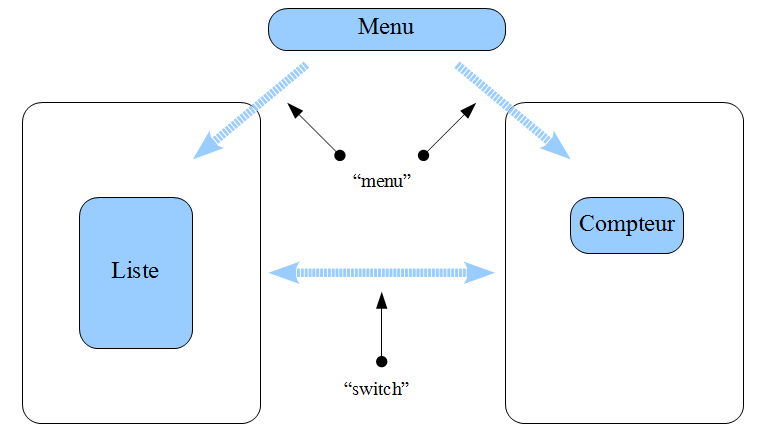
\includegraphics[scale=0.5]{images/modele-relationnel-projet}\caption{Concept relationnel}
\end{figure}
~\\



\subsection{Langages intermédiaires}

Comme nous venons de le voir, la réalisation de notre système passe
par l'introduction de langages intermédiaires liés au dit système
et non à un support logiciel (langage de programmation / OS) ou matériel.
Ceci permet en outre une adaptativité très intéressante.\\



\subsubsection*{Structure de l'interface}

La librairie graphique sera disponible dans un langage de haut niveau
facilitant son utilisation et l'élaboration d'une interface graphique
possiblement complexe, langage qui sera donc dédié à la description
de la structure de l'interface. La librairie fournira donc tous les
outils nécessaires à la définition des actions possibles et à la création
des composants graphiques de l'application, mais aussi des relations
qui les connectent.

De ce point de vue, la librairie sera aussi riche que possible : de
nombreux éléments de base seront donc mis à disposition des développeurs,
et il sera bien évidemment possible (et encouragé) de les composer
ou de les étendre au besoin ; les relations seront également aussi
large que possible, afin d'inclure autant de possibilité que nous
pourrons l'imaginer.\\


Dans cette même logique de réutilisation de l'existant, une autre
volonté de notre part est de permettre la sauvegarde de la structure
d'une interface. Une description indépendante du support logiciel
et matériel de l'interface permet la réalisation de ces objectifs. 

Le but est d’obtenir, après interprétation de la déclaration de structure
de l'interface, un graphe représentant les relations entre les éléments.
Il est à noter que les arêtes de ce graphe doivent être orientées
et typées.\\


Puisque l'aspect visuel des composants ici définis sera précisé séparément
(voir paragraphe suivant), il faut donc que chaque élément et type
d'élément soit doté d'un nom unique qui permette de l'identifier ;
la librairie s'assurera alors de l'absence de conflit pouvant mener
à une confusion entre éléments.\\



\subsubsection*{Aspect visuel}

En revanche, l'aspect de l'interface sera défini séparément, dans
un autre langage. Il s'agit là de lister et préciser des propriétés
de chacun des éléments graphiques utilisés : placement, taille, aspect,
couleurs, effets, espacements, police des textes, etc. Ce langage
doit permettre de fixer l'aspect visuel d'une classe de composant,
affectant ainsi tout composant de ce type utilisé dans l'application,
et aussi de modifier plus finement encore les valeurs d'un élément
en particulier.

Cette feuille de style va compléter notre solution à base de modèle
relationnel et nous permettre d'obtenir l'adaptabilité recherchée.\\


À cette fin, un langage de script, inspiré du \textsc{css} utilisé
en programmation web, doit suffire. Un tel langage permet à chacun,
même sans connaissance de programmation ou de la bibliothèque graphique,
de modifier aisément la feuille de style d'une application à sa convenance.
De plus, toutes ces informations étant de fait regroupées dans un
fichier texte bien structuré et au format spécifié, il est également
possible de coder un programme graphique pour lire et modifier à la
volée les propriétés d'une interface à destination de l'utilisateur
final, laissant à chacun le soin de configurer aussi finement que
possible son interface. 

Puisque de nombreuses feuilles de style différentes peuvent donc être
définies pour une même interface, on laissera la possibilité d'enregistrer
plusieurs de ces configurations et d'en changer à la volée.\\


L'utilisation de cet outil permet d'adjoindre à une même interface
un comportement, un agencement et un visuel par défaut propre à chaque
support : selon le système d'exploitation, le support physique (tablette
ou ordinateur), ou la taille de l'écran, par exemple. Il permet également
au programmeur d’établir une charte graphique unique pour toutes ses
applications, et ce sans avoir à s'en préoccuper à chaque nouveau
projet.

Un choix est à faire à ce niveau, l'utilisation d'un comportement
par défaut lié à un support permet à l'application de se \og fondre \fg{}
dans l'écosystème du support considéré, alors que l'utilisation d'un
style commun à plusieurs projets mais relativement indépendant des
chartes graphiques établies pour chaque support permet de créer une
identité visuelle pour tout un groupe d'applications.\\


Enfin, la librairie doit bien évidemment disposer d'une politique
intelligente et cohérente de valeurs par défaut pour chacun des composants,
permettant d'obtenir une interface fonctionnelle et agréable même
en l'absence de redéfinition de ces propriétés, mais la possibilité
doit également être offerte de les modifier à volonté.\\


Par ailleurs la librairie graphique doit proposer une analyse statique
forte de la feuille de style associée à une interface : les erreurs
qui s'y glissent doivent apparaître dès la compilation, telles que
:
\begin{itemize}
\item des références à des composants graphiques n'existant pas dans l'interface
considérée ;
\item des références à des paramètres n'existant pas pour le composant dans
lequel ils sont redéfinis ;
\item des valeurs mal typées ou non autorisées (par exemple, dépassant des
limites fixées pour le paramètre considéré).\\

\end{itemize}
Notons que la distinction entre ce qui doit être défini par l'application
elle-même (via la librairie, dans le langage dans lequel elle est
définie) ou dans ce langage de script est parfois mince. Par exemple,
dans le cas d'une barre d'outils, c'est au développeur de coder les
éléments qui peuvent y figurer ; mais la configuration de la barre
d'outil finale peut être affinée dans le langage de script en y précisant,
parmi ces éléments, lesquels sont effectivement inclus et dans quel
ordre.\\



\subsubsection*{Exemple suivi}

La description de la structure a déjà été évoquée lors de l'application
à l'exemple du modèle relationnel. Nous avons un menu, deux panneaux,
un afficheur de liste et un afficheur de compteur.\\
Le menu est lié par \og menu \fg{} à chacun des panneaux, c'est
une relation orientée du menu vers le panneau ciblé.\\
Les deux panneaux sont liés par \og switch \fg{}, qui est une relation
orientée aussi, mais ici nous l'utilisons dans les deux sens.\\
Nous omettons volontairement la fenêtre qui n'a pas grand intérêt
ici, elle sert de conteneur à l'ensemble.
\end{document}
